\section{Deep Neural Networks}

Deep learning is a subset of ml and ai, where the models try to process information like the human mind CITE. Since its' beginnings in 1950s with MLPs, deep learning

Deep neural networks work on a layer to layer basis. The formula for computation between two layers is as follows:



The major bottleneck of all kinds of machine learning tecniques is data. The more diverse and varied a .

When it comes to \acrshort{ai} and \acrshort{ml} we usually differentiate between tree major types, those being supervised, unsupervised and semi-supervised learning (or self-supervised learning). They differ in the roles that can occur.


\subsection{Linear Layers}
\label{back:linear}

Fully Connected Layer, Dense Layer or Linear Layers  are types of an operation used in several deep learning models. This layer take an input vector and maps it to an output of learnable parameters. The resulting parameters are thus a weight matrix $W$ and a bias vector $b$. It is defined as follows:

\begin{align}
    Y &= WX + b
\end{align}

where:
\begin{align*}
    X & \text{ - input vector [$n x m$] where $m$ is the amount of input features and $n$ is the batch size} \\
    W & \text{ - weight matrix [$m x p$] where $p$ is the amount of output features} \\
    b & \text{ - bias vector of size $p$} \\
    Y & \text{ - output vector [$n x p$]} \\
\end{align*}

\begin{figure}[h]
    \centering
    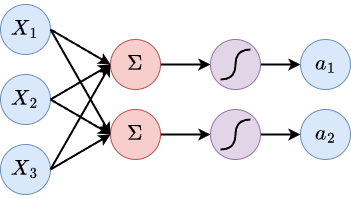
\includegraphics[width=0.5\linewidth]{figures/linearlayer.png}
    \caption{Example of a $3x2$ linear layer}
    \label{fig:linearlayer}
\end{figure}

Furthermore, an activation function such as \gls{relu} \ref{eq:relu} is applied to the output to achieve nonlinearity.
Lets denote this function as $f$, we now get the following equation.

\begin{equation}
    Z = f(Y) = f(XW+b)
\end{equation}

Linear layers have several advantages, such as computational efficiency, flexibility as well as intrerprebility, where the weight and bias vectors can be interpreted as learned parameters. They also serve as building blocks for other components, such as \acrshort{rnn}s, \acrshort{lstm}s or even attention blocks. \\ 

However, linear layers have several limitations. Due to their inherent linearity, they are prone to overfitting and struggle to capture complex relationships in data. This can limit their ability to extract more complex features, potentially reducing some of the model's discriminative power. Furthermore, the size of linear layers can become problematic, especially in fully connected dense neural networks. Each neuraon connection between layers requires storing weights and biases, which increases the overall model size. This can create bottlenecks for many hardware accelerators, such as \acrshort{gpu}s, when dealing with large models.

\subsubsection{Early Stopping}

Overfitting is a common problem within \acrlong{ml}. It occurs when a model is trained , and fails to fit additional data. \textit{Early Stopping} is a regularization technique that aims to avoid such issue. When training an optimizer, such as \acrshort{adam} or \acrshort{sgd}, we can notice when a model is overfitting by studying the validation loss. If we notice an increase of validation loss, the early stop mechanism will stop the training altogether if no improvement of optimal validation loss is found after $p$ amount of epochs. The validation loss is commonly used to evaluate the hyperparameters of a model, and ac 


\begin{align*}
&\text{Stop at epoch } T \text{ if:} \\
&\forall i \in \{T-p+1, ..., T\}: L_t(i) > L_t^* - \epsilon \\
&\text{where } L_t^* = \min_{j=1}^{T} L_t(j) \\
\\
&\text{Given:} \\
&L_t(t) \text{ is the train loss at epoch } t \\
&p \text{ is the patience (number of epochs to wait)} \\
&\epsilon \text{ is a small threshold for improvement}
\end{align*}

\subsection{Parallelism within \acrlong{ml}}

With rapid evolving deep learning architectures, the importance of scalable model training and networks grows larger each year. It is even estimated that these networks grow 1,5x each year \cite{9499913}, making parallelization a vital topic when it comes to \acrlong{ml} to accommodate ever increasing memory needs. Several different hardware accelerators have been created to best accommodate these needs, the most apparent of these are \acrshort{gpu}s. NVIDIA have for several years dominated this market, and their hardware is becoming faster and increasing in memory. \\

By workers, we mainly refer to \acrshort{gpu}s, but this could also be processors or other types of hardware accelerators such as TPUs.


\subsubsection{Model Parallelism}

Deep learning models need to store a lot of data. Weights and biases tend to take up a lot of memory, thus requiring the need of splitting up a model across several workers. As an example, given a model $M$ of 50 layers, we can split this model in 2 parts by having a worker $A$ manage the first 25 layers, and worker $B$ manage the latter half.

The overhead of transferring data across these workers can become a bottleneck, so this should only be utilized when absolutely necessary.

\subsubsection{Data Parallelism}

Data parallelism refers to partitioning data across multiple workers.  Given a large set of data, we can split these data across the workers and store a copy of the model on each worker, calculate gradients across them all and update the trainable parameters for the model. An example of this would be to split a batch of size $b$ across $n$ workers, calculate the gradients and update the model. Before updating the parameters of the model, an average across all parameters is calculated, and each of the copies of the model is updated before continuing.

\subsubsection{Hybrid Parallelism}

This kind of parallelization is a combination of the two previously mentioned techniques. By first splitting a model across several workers, data is subsequently split across multiple workers. 

\subsection{CNN - Convolutional Neural Networks}
\label{back:cnn}

\acrfull{cnn}, a specialized type of feed-forward neural network, has become a cornerstone in \acrshort{dl} architectures. Building upon simpler structures like the linear layer discussed in section \ref{back:linear}, CNNs introduce a powerful approach to processing matrix data, especially images.
The foundations of CNNs can be traced back to neurobiological research in the 1960s on the visual cortex \cite{hubel1962receptive}, but they were first properly introduced to the \acrshort{ml} field in 1989 by LeCun et al. \cite{NIPS1989_53c3bce6}. Since then, CNNs have undergone significant developments, leading to breakthroughs in various fields of artificial intelligence. \\

\begin{figure}[!h]
    \centering
    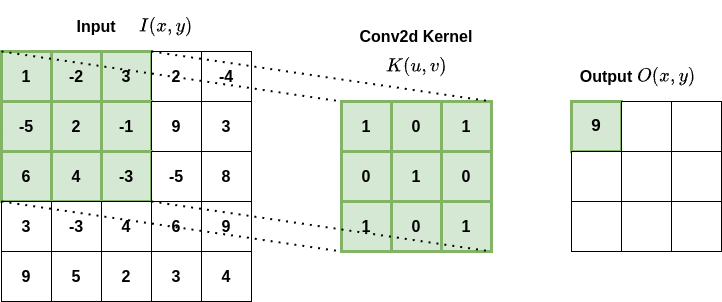
\includegraphics[width=0.8\linewidth]{figures/convolution.png}
    \caption{Example of a 2D Convolutional operation}
    \label{fig:2dconv}
\end{figure}

At their core, CNNs rely on kernel operations, primarily convolutions, to calculate features. The convolution is a mathematically operation which can be defined continuously as following:

\begin{equation}
(f * g)(t) = \int_{-\infty}^{\infty} f(\tau) g(t - \tau) d\tau
\label{eq:contconv}
\end{equation}

and discretely as such:

\begin{equation}
   (f * g)(x, y) = \sum_{m=0}^{M-1} \sum_{n=0}^{N-1} f(m, n)g(x-m, y-n) 
\label{eq:conv}
\end{equation}

The convolutional operation is essentially multiple matrix multiplication between different regions in the data and a kernel. These multiplications can be performed in a parallelized manner. Matrix multiplications have undergone significant improvement over the years CITE, and have with the introduction of CUDA, been further optimized for better suited hardware architectures such as \acrshort{gpu}s. With the rapid improvements of \acrshort{gpu}s, especially by NVIDIA, the computational efficiency of both linear and convolutional layers has improved drastically. This has resulted in overall lower energy requirements for model training, reduced training times and the introduction of distributed large-scale model training \cite{mungoli2023scalable}. \\ 

Unlike fully connected layers that compute global interactions, convolution operations in CNNs focus on local regions data. This localized approach allows for improved feature extraction, making them particularly effective for tasks involving spatial data such as image recognition, object detection, and segmentation. \\



The power of CNNs lies in their ability to automatically learn hierarchical feature representations. Lower layers typically detect simple features like edges or colors, while deeper layers combine these to recognize more complex features. This hierarchical learning, coupled with parameter sharing and local connectivity, enables CNNs to be both computationally efficient and highly effective at capturing relevant features from high-dimensional data. \\

Due to \acrshort{cnn}s inherent quality of feature extraction, they are not as prone to the vanishing gradient problem as linear layers. This occurs when gradients propagated backward through the layers become very small, making it difficult for the network to update its weights effectively. \\

Only the size of the kernel is used to stored neurons when performing cross correlation convolution, compared to linear layers where all the weights between layers needs to be stored. \acrshort{cnn}s are highly applicable to numerous different tasks, such as recognition and classification. \\

\subsubsection{Pooling}

Typically, a convolution is followed by an activation function and then a pooling operation. A pooling operation works like a filter $f$, selecting a certain value from a set of numbers based on a measurement. The three most common operations are \textit{max pool}, \textit{min pool} and \textit{avg pool}. Out of these, the \textit{max pool} operation operation is most commonly used. This operation reduces dimensionality, outputting only the most important feature for future layers. \\

\begin{figure}[!h]
    \centering
    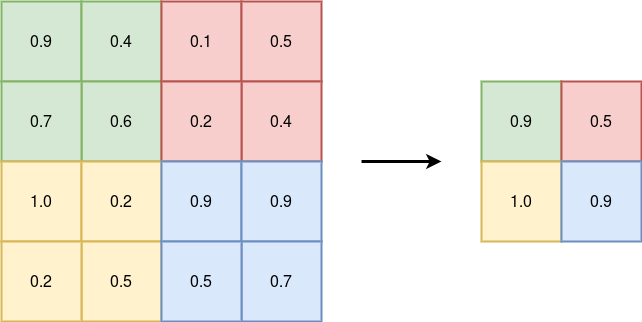
\includegraphics[scale=0.4]{figures/pooling.png}
    \caption{Example of a $2 x 2$ max pool operation with stride 2}
    \label{fig:maxpool}
\end{figure}